%!TEX root = thesis.tex
\chapter{Demonstrator}
\label{sec:demo}

\section{Stewart Platform}
The Stewart platform was introduced by D. Stewart in 1965 \citep{Ste65} and
gained popular resarch interest in robotics \citep{Szu13}, concerning
kinematics, dynamics or work space estimations. However, outside the
scientific community the Stewart platform was not widely adopted and most
designs are constrained to applications requiring \ac{6DoF}, for instance
flight simulators or \ac{CNC} machining centers. Although a Stewart platform
provides many potential advantages , sophisticated synthesis and simulation
tools are missing \citep{Ji96}. Against the background of increasing
computational capabilities and more efficient \ac{CAD} tools, this situation
might change in the future. In the scope of this thesis, the Stewart platform
promises to be a sophisticated development platform, involving computationally
expensive calculations for its kinematics and additional I/O capabilities.
Therefore, it seems to be a suitable demonstrator for a modern \acp{PAC}.

The following sections introduce the architecture of the Stewart platform in
general and the variant used in this thesis, specifying the used notation and
solving the inverse kinematics problem.

\subsection{Architecture}
While Stewart introduced the general idea of a Stewart platform in his work in
1965 \citep{Ste65}, a strict definition is missing in the literature. The only
commonality is the characterization as a parallel manipulator \citep{Szu13}
consisting out of a bottom base and an upper platform. Compared to a serial
manipulator, it consists out of multiple serial chains controlled
simultaneously and connected to a single end-effector. While this design
provides unique benefits like high accuracy, better load-to-weight ratios and
improved rigidity, it limits the available work space and causes highly
nonlinear behavior.

Figure \ref{fig:stewart_architectures} illustrates different variants of
Stewart platforms found in the literature.
\begin{figure}
	\centering
	\begin{subfigure}{0.3\textwidth}
		\centering
		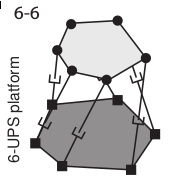
\includegraphics[width=\textwidth]{../figures/stewart_architectures_c}
		\caption{6-UPS}
		\label{fig:stewart_architectures_a}
	\end{subfigure}
	\begin{subfigure}{0.3\textwidth}
		\centering
		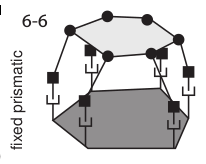
\includegraphics[width=\textwidth]{../figures/stewart_architectures_d}
		\caption{Fixed prismatic}
		\label{fig:stewart_architectures_b}
	\end{subfigure}
	\begin{subfigure}{0.3\textwidth}
		\centering
		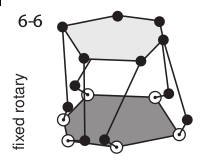
\includegraphics[width=\textwidth]{../figures/stewart_architectures_e}
		\caption{Fixed rotary}
		\label{fig:stewart_architectures_c}
	\end{subfigure}
	\caption{Different variants of Stewart platforms \citep[adopted from][]{Szu13}}
	\label{fig:stewart_architectures}
\end{figure}
They vary in the type of the connections and actuators, as well as their
spacial configuration, i.e. the positioning of the different connections.
Figure \ref{fig:stewart_architectures_a} shows the most common realization
using six prismatic actuator, for example hydraulic pistons or linear motors.
This variant is often referred to as Hexapod and associated with the term
Stewart platform, not least because of its similarity to the original design
proposed by Stewart. Other architectures utilize fixed prismatic actuators as
shown in figure \ref{fig:stewart_architectures_b} or rotary actuators as
illustrated in figure \ref{fig:stewart_architectures_c}. All of these variants
have its unique benefits and drawbacks. Since the actuators in the latter
design can be realizing as commonly available servo motors, it gained
popularity, especially for low-cost designs and first prototypes. Therefore,
this thesis focuses on a servo-based architecture as shown in figure
\ref{fig:stewart}. The mechanical design and construction was not focused in
this thesis, but reused from a previous work.
\begin{figure}[tb]
	\centering
	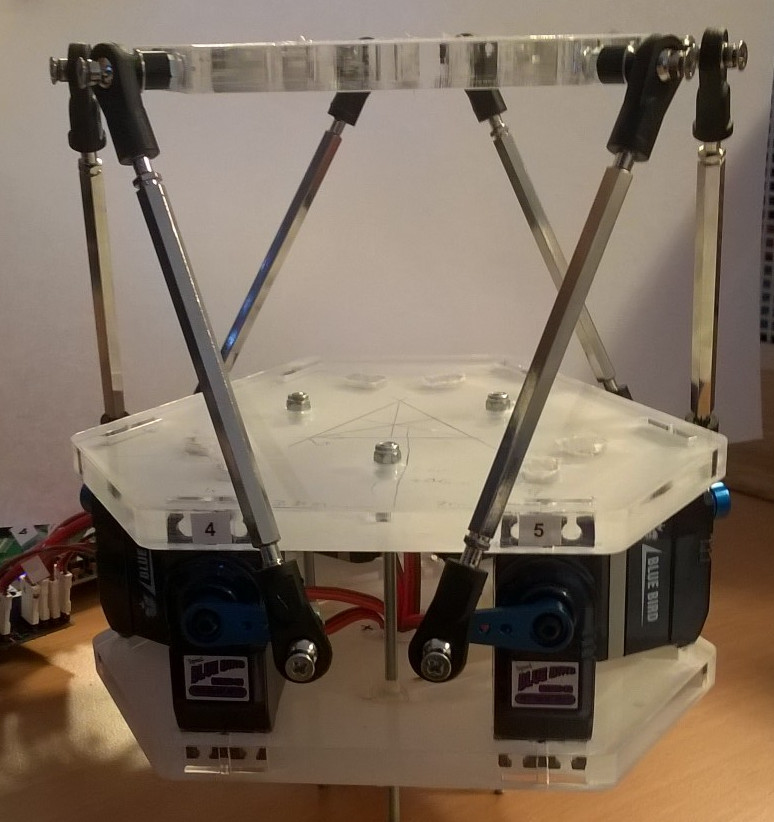
\includegraphics[width=6cm]{../figures/stewart}
	\caption{Construction of the Stewart platform prototype}
	\label{fig:stewart}
\end{figure}

\subsection{Construction and Notation}

\subsection{Inverse Kinematics}